
%
\begin{frame}
\frametitle{}
\begin{center}
  \textbf{\Large The Shuffled Complex Evolution}
\end{center}
\end{frame}

%
\begin{frame}
\frametitle{The Shuffled Complex Evolution}
\begin{columns}
\begin{column}{0.75\textwidth}  %%<--- here
  {\small
  The SCE  regards a natural  evolution happening
  simultaneously in independent communities;
  \\ \medskip \pause
  A population of $N*M$ individuals is randomly taken from the
  solution space;
  \\ \medskip \pause
  The population is then sorted by descending order of fitness
  and the best global solution is identified;
  \\ \medskip \pause
  The population is then shuffled into $N$ complexes,
  each containing $M$ individuals;
  \\ \medskip \pause
  In this shuffling process the first individual goes to the first complex, the second
  individual goes to the second complex, individual $N$ goes to $N$-th complex,
  individual $(M+1)$-th goes back to the first complex, etc;
  \\ \medskip \pause
  The next step after shuffling the complexes is to evolve each complex.
  }
\end{column} \pause
\begin{column}{0.25\textwidth}
  \hspace{-15pt}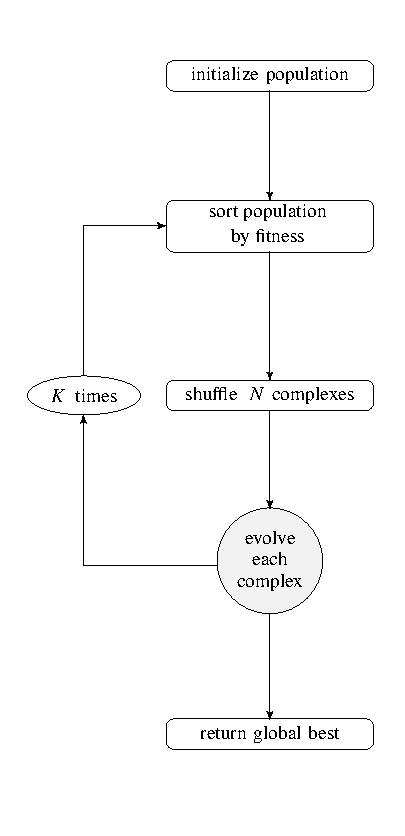
\includegraphics[scale=0.45]{img/sce/flow1}
\end{column}
\end{columns}
\end{frame}

%
\begin{frame}
\frametitle{The Shuffled Complex Evolution}
\begin{columns}
\begin{column}{0.75\textwidth}  %%<--- here
  {\small
  In each step a subcomplex of $P$ individuals is selected from the
  complex;
  \\ \medskip \pause
  After the selection of the subcomplex, its worst individual is identified to
  be replaced by a new generated solution;
  \\ \medskip \pause
  This new solution is generated by the crossing of the worst individual and an
  other individual with better fitness;
  \\ \medskip \pause
  At first the best individual of the subcomplex is considered for the crossing;
  \\ \medskip \pause
  If the new solution is not better than the worst one, the best individual
  of the complex is considered for a crossing;
  \\ \medskip \pause
  If the latter crossing did not result in any improvement, the best individual
  of whole population is considered;
  \\ \medskip \pause
  Finally, if all the crossing steps couldn't generate a better individual,
  the worst individual of the subcomplex is replaced by a new random solution taken
  from the feasible solution space.
  }
\end{column} \pause
\begin{column}{0.25\textwidth}
  \vspace{10pt}\hspace{-18pt}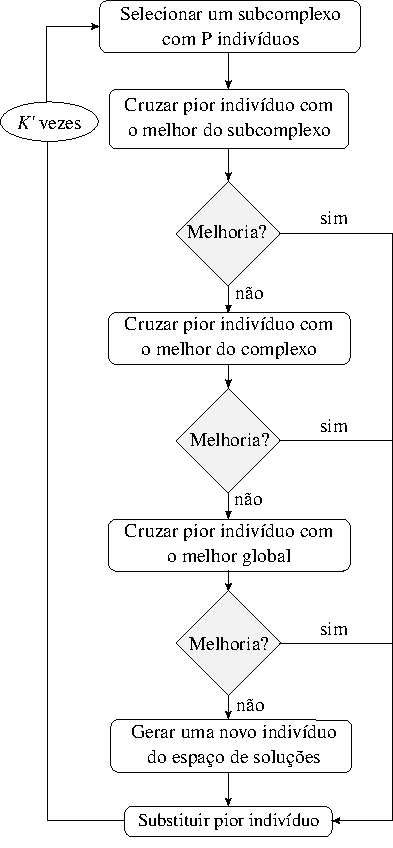
\includegraphics[scale=0.45]{img/sce/flow2}
\end{column}
\end{columns}
\end{frame}

%
\begin{frame}
\frametitle{}
\begin{center}
  \textbf{\Large The Shuffled Complex Evolution}
  \\ \bigskip \bigskip
  {\large Use case for the MKP}
\end{center}
\end{frame}

% The SCE for MKP
\begin{frame}
\frametitle{The SCE for MKP}
the SCE is easily applied to any
optimization problem.
The only steps needed to be specified is \textbf{(a)} the creation of a new random
solution and \textbf{(b)} the crossing procedure of two solutions.
\end{frame}

% Random for MKP
\begin{frame}
\frametitle{The SCE for MKP}
New random solution generation for the MKP.
\begin{figure}
\begin{algorithmic}[1]
  \Function{New random solution}{} \pause
    \State $v \leftarrow $ shuffle($1, 2, \ldots, n$) \pause
	\State $s \leftarrow \emptyset$ \pause
    \For{$ i \leftarrow 1:n$ }
	  \State $s \leftarrow s \cup \{v_i\}$ \pause
	  \If{ $s$ is not feasible} \pause
	    \State $s \leftarrow s - \{v_i\}$
      \EndIf  \pause
	\EndFor
  \State return $s$
  \EndFunction
\end{algorithmic}
\end{figure}
\end{frame}

% Crossing for MKP
\begin{frame}
\frametitle{The SCE for MKP}
Crossing procedure for the MKP.
\begin{figure}
\begin{algorithmic}[1]
  \Function{Crossing}{$x^w:$ worst individual, $x^b:$ better individual, $c$} \pause
    \State $v \leftarrow $ shuffle($1, 2, \ldots, n$) \pause
    \For{$ i \leftarrow 1:c$ }
	  \State $j \leftarrow v_i$ \pause
	  \State $x^w_j \leftarrow x^b_j$
	\EndFor \pause
	\If{$s^w$ is not feasible}
	  \State repair $s^w$
	\EndIf \pause
  \State return $s^w$
  \EndFunction
\end{algorithmic}
\end{figure}
\end{frame}


% SCE parameters
\begin{frame}
\frametitle{Computational Experiments}
Parameters used for SCE:
\begin{itemize}
  \item $N = 20$: number of complexes;
  \item $M = 20$: number of individuals in each complex;
  \item $P = 5$: number of individuals in each subcomplex;
  \item $K = 300$: number of algorithm iterations;
  \item $K' = 20$: number of iterations used in the complex evolving process;
  \item $c = n/5$: number of genes carried from parent in crossing process.
\end{itemize}
\end{frame}

% Results (chub)
\begin{frame}
\frametitle{Computational Experiments}
SCE and \scecore  performance on Chu-Beasley problems.
\begin{table}[hb]
{
\renewcommand{\arraystretch}{0.7}%
\fontsize{4.5pt}{1em}\selectfont
\begin{center}
  \begin{tabular}{rrr|cc|cc} \hline
  \multirow{2}{*}{\bf n} &
  \multirow{2}{*}{\bf m} &
  \multirow{2}{*}{\textbf{$\alpha$}} &
    \multicolumn{2}{c|}{\textbf{time} (s)} &
    \multicolumn{2}{c}{\textbf{quality}(\%)} \\
  &
    &
    &
    \textbf{SCE} &
    \textbf{\scecore} &
    \textbf{SCE} &
    {\bf \scecore}  \\ \hline
100   &  5 & 0.25 & 1.22\fvar{0.04} & \textbf{0.17}\fvar{0.00} & 96.51\fvar{0.92} & \textbf{99.73}\fvar{0.04} \\
        &    & 0.50 & 1.34\fvar{0.02} & \textbf{0.18}\fvar{0.00} & 97.42\fvar{0.55} & \textbf{99.86}\fvar{0.01} \\
        &    & 0.75 & 1.37\fvar{0.03} & \textbf{0.17}\fvar{0.00} & 98.87\fvar{0.20} & \textbf{99.91}\fvar{0.00} \\ \cline{2-7}
        & 10 & 0.25 & 1.32\fvar{0.04} & \textbf{0.25}\fvar{0.00} & 95.68\fvar{1.28} & \textbf{99.53}\fvar{0.09} \\
        &    & 0.50 & 1.51\fvar{0.04} & \textbf{0.25}\fvar{0.00} & 96.65\fvar{0.49} & \textbf{99.76}\fvar{0.03} \\
        &    & 0.75 & 1.46\fvar{0.04} & \textbf{0.27}\fvar{0.00} & 98.54\fvar{0.19} & \textbf{99.96}\fvar{0.00} \\ \cline{2-7}
        & 30 & 0.25 & 1.74\fvar{0.06} & \textbf{1.20}\fvar{0.03} & 95.38\fvar{1.01} & \textbf{97.96}\fvar{0.22} \\
        &    & 0.50 & 1.79\fvar{0.08} & \textbf{0.89}\fvar{0.06} & 96.41\fvar{0.63} & \textbf{99.18}\fvar{0.06} \\
        &    & 0.75 & 1.72\fvar{0.09} & \textbf{0.95}\fvar{0.04} & 98.18\fvar{0.33} & \textbf{99.52}\fvar{0.04} \\ \hline
\multirow{2}{*}{250} & 5 & 0.25 & 2.87\fvar{0.07} & \textbf{0.69}\fvar{0.01} & 93.22\fvar{0.64} & \textbf{99.86}\fvar{0.00} \\
        &    & 0.50 & 2.82\fvar{0.11} & \textbf{0.70}\fvar{0.01} & 94.88\fvar{0.21} & \textbf{99.94}\fvar{0.00} \\
        &    & 0.75 & 2.93\fvar{0.08} & \textbf{0.69}\fvar{0.01} & 97.57\fvar{0.10} & \textbf{99.96}\fvar{0.00} \\ \cline{2-7}
        & 10 & 0.25 & 3.08\fvar{0.09} & \textbf{0.87}\fvar{0.01} & 93.14\fvar{0.67} & \textbf{99.58}\fvar{0.01} \\
        &    & 0.50 & 3.03\fvar{0.09} & \textbf{0.79}\fvar{0.02} & 94.55\fvar{0.26} & \textbf{99.79}\fvar{0.00} \\
        &    & 0.75 & 3.12\fvar{0.09} & \textbf{0.84}\fvar{0.01} & 97.16\fvar{0.13} & \textbf{99.88}\fvar{0.00} \\ \cline{2-7}
        & 30 & 0.25 & 3.74\fvar{0.12} & \textbf{1.52}\fvar{0.04} & 93.10\fvar{0.74} & \textbf{98.42}\fvar{0.08} \\
        &    & 0.50 & 3.74\fvar{0.16} & \textbf{1.36}\fvar{0.06} & 94.20\fvar{0.30} & \textbf{99.33}\fvar{0.02} \\
        &    & 0.75 & 3.99\fvar{0.13} & \textbf{1.48}\fvar{0.04} & 96.64\fvar{0.14} & \textbf{99.59}\fvar{0.01} \\ \hline
\multirow{2}{*}{500} & 5 & 0.25 & 5.62\fvar{0.10} & \textbf{1.25}\fvar{0.02} & 91.37\fvar{0.50} & \textbf{99.77}\fvar{0.00} \\
        &    & 0.50 & 5.72\fvar{0.19} & \textbf{1.24}\fvar{0.01} & 93.39\fvar{0.27} & \textbf{99.88}\fvar{0.00} \\
        &    & 0.75 & 5.88\fvar{0.14} & \textbf{1.20}\fvar{0.02} & 96.42\fvar{0.06} & \textbf{99.92}\fvar{0.00} \\ \cline{2-7}
        & 10 & 0.25 & 5.97\fvar{0.17} & \textbf{1.41}\fvar{0.02} & 91.62\fvar{0.50} & \textbf{99.51}\fvar{0.01} \\
        &    & 0.50 & 6.11\fvar{0.23} & \textbf{1.36}\fvar{0.03} & 93.09\fvar{0.20} & \textbf{99.77}\fvar{0.00} \\
        &    & 0.75 & 5.47\fvar{0.61} & \textbf{1.21}\fvar{0.03} & 96.24\fvar{0.06} & \textbf{99.84}\fvar{0.00} \\ \cline{2-7}
        & 30 & 0.25 & 6.20\fvar{1.14} & \textbf{1.96}\fvar{0.22} & 91.37\fvar{0.82} & \textbf{98.76}\fvar{0.02} \\
        &    & 0.50 & 6.26\fvar{1.07} & \textbf{1.82}\fvar{0.14} & 92.56\fvar{0.13} & \textbf{99.42}\fvar{0.01} \\
        &    & 0.75 & 6.05\fvar{1.16} & \textbf{1.73}\fvar{0.20} & 95.97\fvar{0.06} & \textbf{99.67}\fvar{0.00} \\ \hline
\end{tabular}

\end{center}
}
\end{table}
\end{frame}

% Results (gk)
\begin{frame}
\frametitle{Computational Experiments}
\scecore performance on Glover-Kochenberger problems.
\begin{table}[hb]
  {
  \renewcommand{\arraystretch}{1}%
  \fontsize{5.5pt}{1em}\selectfont
  \begin{center}
    \begin{tabular}{rrr|cc|rr} \hline
  \multirow{2}{*}{\textbf{\#}} &
  \multirow{2}{*}{\textbf{n}} &
  \multirow{2}{*}{\textbf{m}} &
    \multicolumn{2}{c|}{\textbf{time}(s)} &
    \multicolumn{2}{c}{\textbf{quality}(\%)} \\
  &
    &
    &
    \textbf{SCE} &
    \textbf{SCEcr} &
    \textbf{SCE} &
    \textbf{SCEcr} \\ \hline
  01   &  100 &  15 &   1.47\fvar{0.00} & \textbf{0.08}\fvar{0.0} & 97.66\fvar{0.03} & \textbf{99.24}\fvar{0.02} \\ \hline
    02 &  100 &  25 &   1.61\fvar{0.00} & \textbf{0.09}\fvar{0.0} & 97.94\fvar{0.04} & \textbf{98.94}\fvar{0.09} \\ \hline
    03 &  150 &  25 &   2.51\fvar{0.01} & \textbf{0.09}\fvar{0.0} & 97.22\fvar{0.04} & \textbf{99.09}\fvar{0.02} \\ \hline
    04 &  150 &  50 &   3.56\fvar{0.03} & \textbf{0.09}\fvar{0.0} & 97.40\fvar{0.04} & \textbf{98.52}\fvar{0.02} \\ \hline
    05 &  200 &  25 &   3.55\fvar{0.01} & \textbf{0.09}\fvar{0.0} & 96.88\fvar{0.03} & \textbf{99.28}\fvar{0.01} \\ \hline
    06 &  200 &  50 &   4.81\fvar{0.09} & \textbf{0.10}\fvar{0.0} & 97.68\fvar{0.02} & \textbf{98.90}\fvar{0.03} \\ \hline
    07 &  500 &  25 &   7.30\fvar{0.09} & \textbf{0.10}\fvar{0.0} & 97.12\fvar{0.01} & \textbf{99.54}\fvar{0.00} \\ \hline
    08 &  500 &  50 &  12.20\fvar{0.47} & \textbf{0.11}\fvar{0.0} & 97.27\fvar{0.01} & \textbf{99.33}\fvar{0.01} \\ \hline
    09 & 1500 &  25 &  24.61\fvar{1.73} & \textbf{0.12}\fvar{0.0} & 95.40\fvar{0.01} & \textbf{98.22}\fvar{0.00} \\ \hline
    10 & 1500 &  50 &  33.79\fvar{2.44} & \textbf{0.13}\fvar{0.0} & 97.50\fvar{0.00} & \textbf{99.64}\fvar{0.00} \\ \hline
    11 & 2500 & 100 & 121.28\fvar{194.74} & \textbf{0.15}\fvar{0.0} & 97.95\fvar{0.00} & \textbf{99.70}\fvar{0.00} \\ \hline
\end{tabular}

  \end{center}
  }
\end{table}
\end{frame}

% Results (gk)
\begin{frame}
\frametitle{Conclusions}
The SCE algorithm for MKP proved to be able to achieve fast
convergence ratio, finding good quality near optimal solutions, demanding small
amount of computational time.
\\ \medskip \pause
The core concept as a variable fixing procedure
proved to be efficient to reduce the size of the problems which provided fast
execution time, producing higher quality solutions.
\\ \medskip \pause
At least $99.02\%$ of best known, in less than $2$ seconds for every instance.
\end{frame}
